\section{Exercise 1}

\section{Answer}
\subsection{1}

starting from the equation of motion, seen in the equation, we obtain the
state space representation as below:

\[
A =
\begin{bmatrix}
	0  	& 		0 		&      1	 	&     0\\
	0 	&     0 		&      0 		&     1\\
	\frac{-(k_1 + k_2)}{m_1} & \frac{k_2}{m_1} & \frac{-c_2}{m_1} & \frac{c_2}{m_1}\\
	\frac{k_2}{m_2} & \frac{-k_2}{m_2} & \frac{c_2}{m_2} & \frac{-c_2}{m_2}
	\end{bmatrix}\quad
	B =
	\begin{bmatrix}
		0\\
		0\\
		\frac{1}{m_1}\\
		0
		\end{bmatrix}\quad
		C =
		\begin{bmatrix}
			1   &  0   &  0  &   0
		\end{bmatrix}
		\]

		\subsection{2}
		Setting $u\,=\,0$

		after having calculated by means of numerical substitution, the value of $P$
		given in the matrix \ref{eq:valuep} is obtained.

		\begin{equation}
			\label{eq:valuep}
			\begin{bmatrix*}[l]
				603.3417	&   -8.5265	&    0.1252	&   -5.0157\\
				-8.5265	&  128.7847	&    2.8368	&    0.6276\\
				0.1252	&    2.8368	&    3.9082	&    0.5233\\
				-5.0157	&    0.6276	&    0.5233	&    1.1363
			\end{bmatrix*}
		\end{equation}



		\subsection{3}

		\subsection{4}

		\begin{figure}
			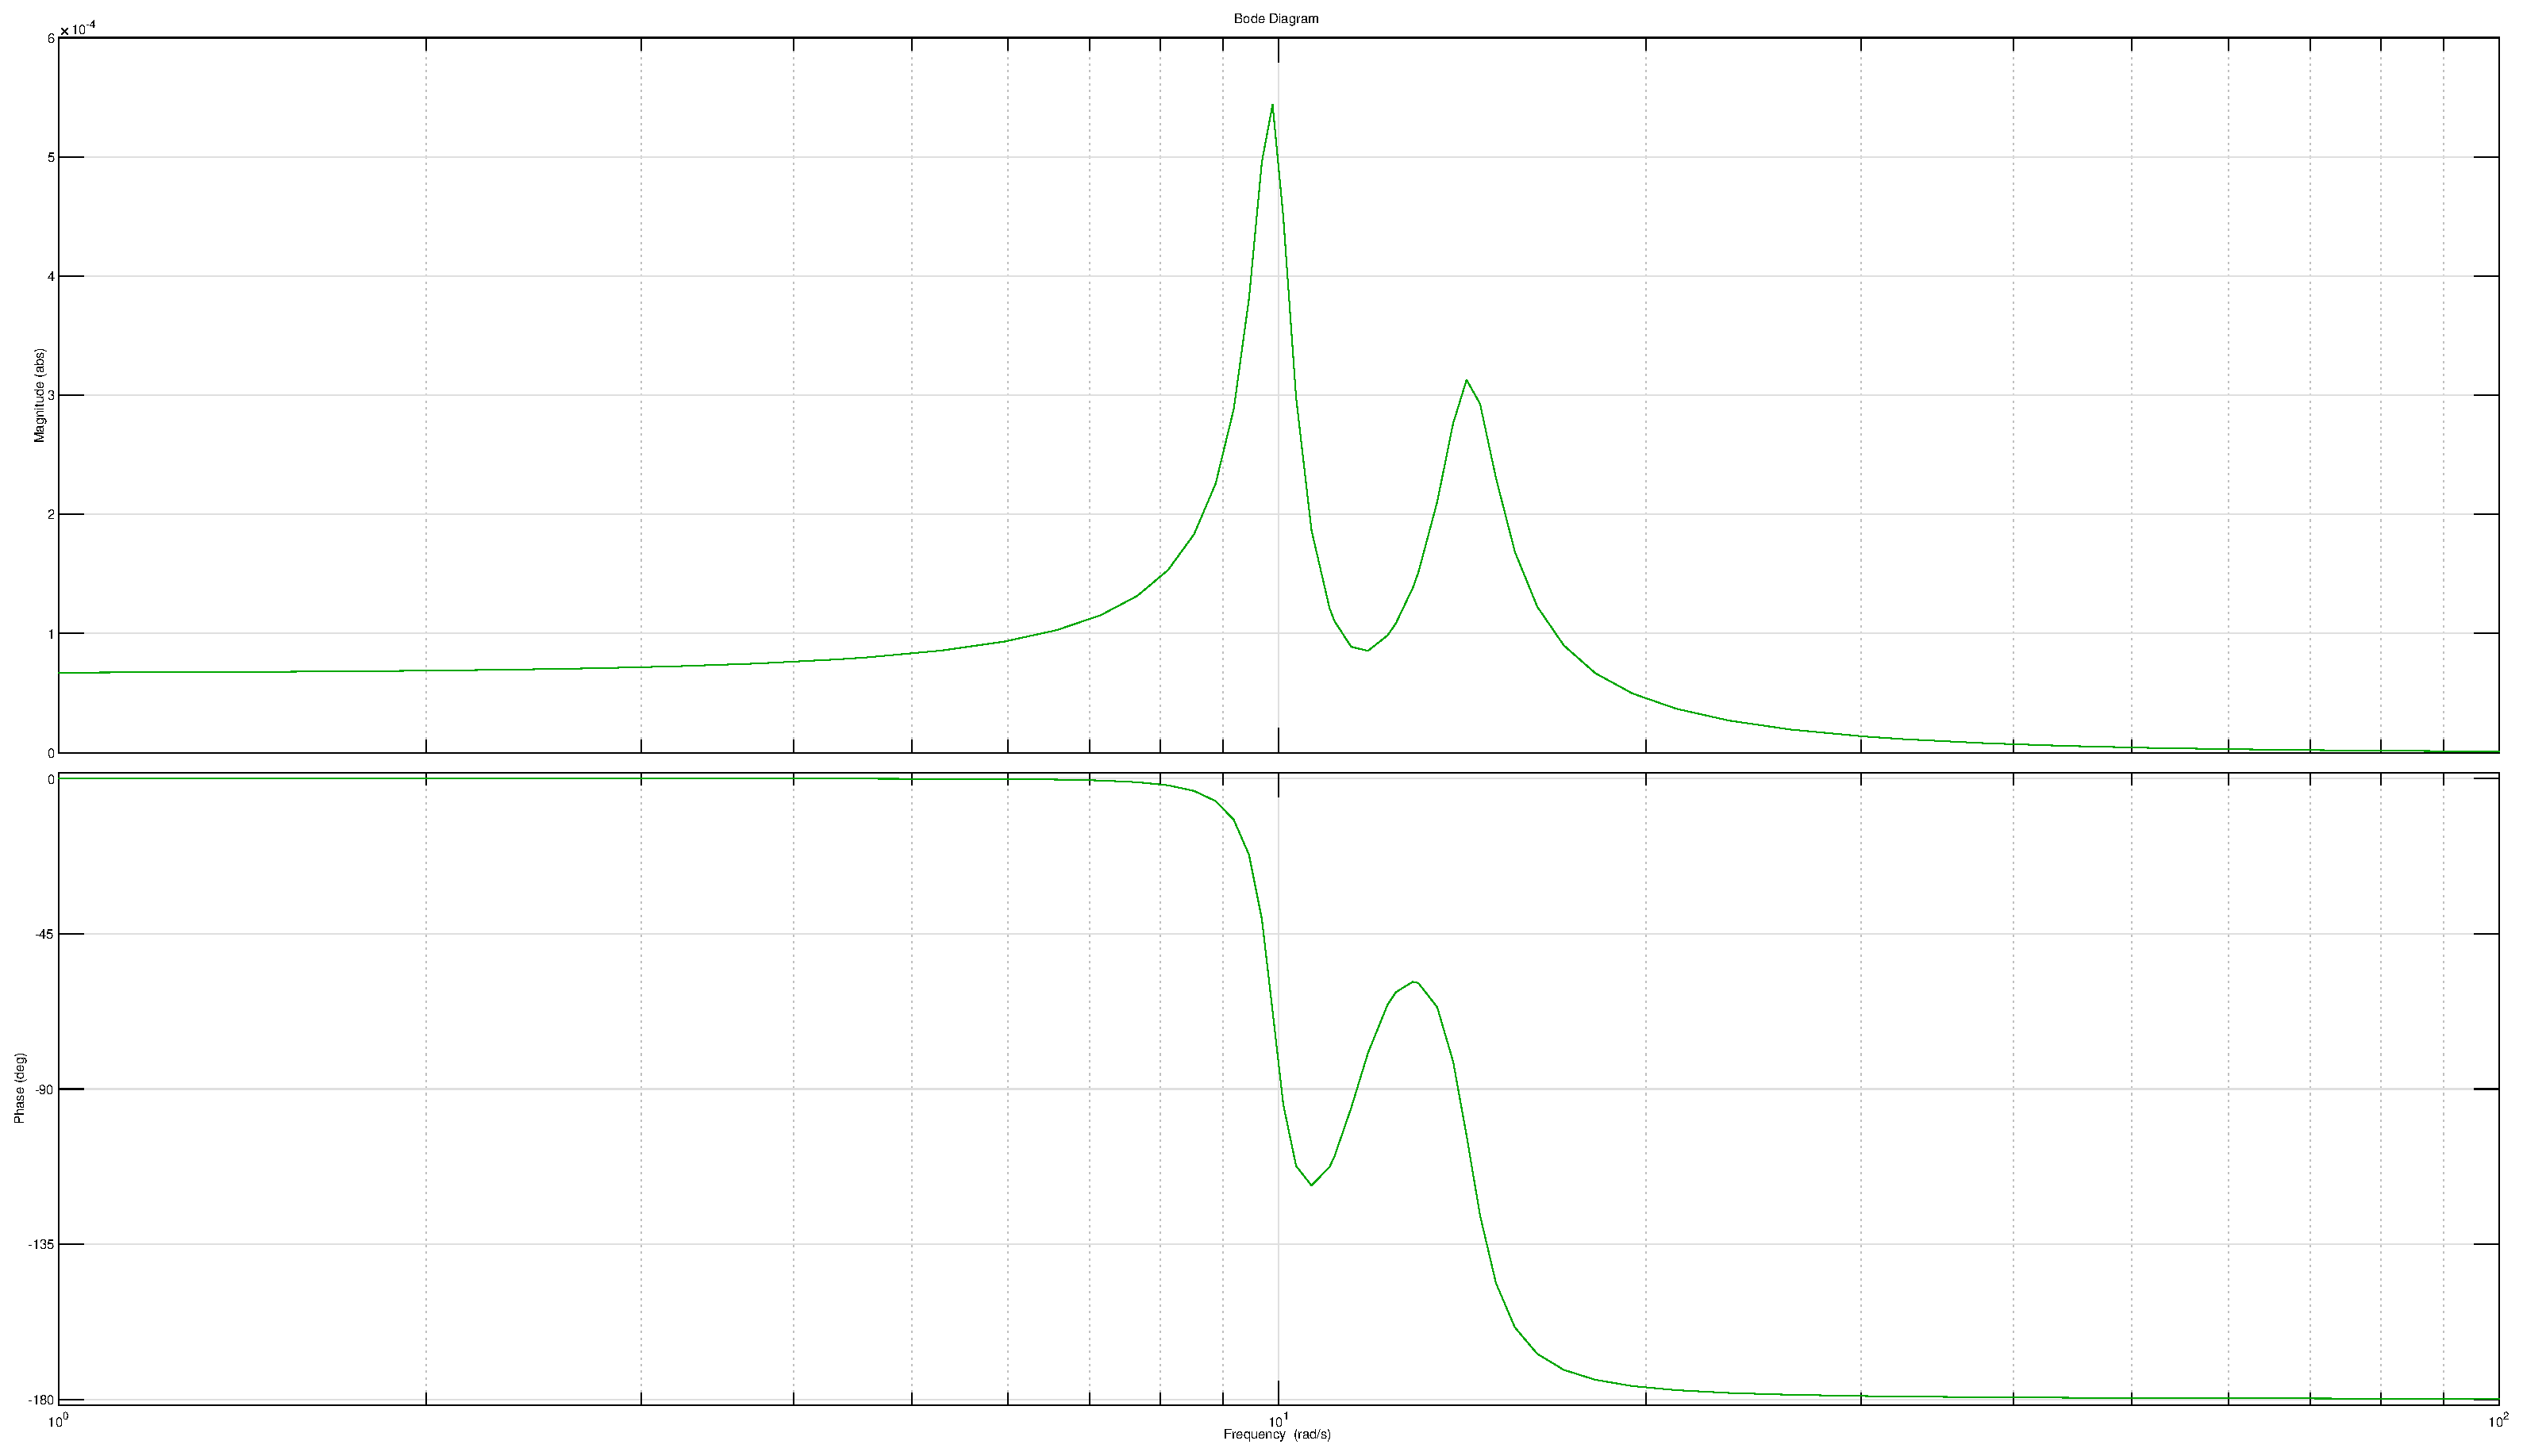
\includegraphics[width=\linewidth]{bode}
			\caption{Bode diagram of tranfer matrix.}
			\label{fig:bodeplot}
		\end{figure}
